\section{Applications}

On présente ici la liste des fonctions de chaque application composant le
SI spécifique conçu pour GSTP.

\begin{figure}[h]
\centering
\caption{Découpage fonctionnel du SI de GSTP}
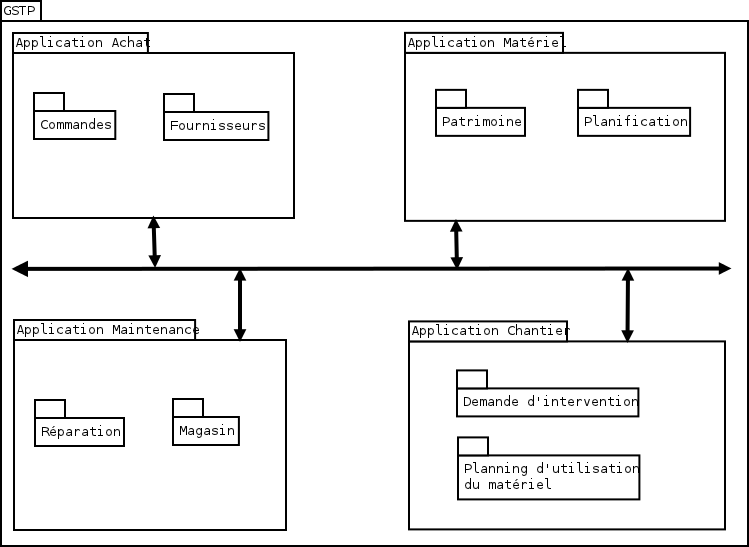
\includegraphics[width=10cm]{\PIXPATH/DecoupageAppli}
\end{figure}


\subsection{Fonctions globales}

L'ensemble des applications utilise une fonctionnalité de {\sl login}, permettant
de restreindre l'accès à certains types d'utilisateurs.


\subsection{Application Achats}
% Communication avec la comptabilité pour les commandes
% Cette fonctionnalité est incluse dans les fonctions de commande, non ?

\begin{itemize}
\item Commander du matériel;
\item Commander des pièces de rechange;
\item Suivre une commande;
\item Suivre le budget;
\item Consulter le catalogue de fournisseurs (recherche de fournisseurs selon 
un ou plusieurs critères);
\item Editer le catalogue de fournisseurs :
	\begin{itemize}
	\item Création d'une fiche fournisseur,
	\item Modification d'une fiche fournisseur,
	\item Suppression d'une fiche fournisseur.
	\end{itemize}
\end{itemize}

\subsection{Application Matériel}
\begin{itemize}
\item Récupérer les plannings prévisionnels d'utilisation de matériels
des chantiers.
\item Établir le planning effectif d'affectation des
matériels pour les chantiers.
\item Calculer et transmettre les factures qui correspondent à chaque chantier
à partir de l'utilisation des matériels.
\item Enregistrer les mouvements de matériels (entrées et sorties du parc).
\item Évaluation de la valeur du parc.
\end{itemize}


\subsection{Application Maintenance}
\subsubsection{Opérations de maintenance}
\begin{itemize}
\item Récupérer l'ensemble des demandes de maintenance exceptionnelle
des matériels.
\item Etablir le planning pour la maintenance du matériel, prenant en
compte les maintenances préventives et curatives :
    \begin{itemize}
    \item planning global,
    \item planning journalier,
    \item anticipation de maintenances curatives.
    \end{itemize}
\item Editer le catalogue et le  journal de maintenance pour chaque matériel :
    \begin{itemize}
    \item Consultation du catalogue de maintenance associé à une classe de 
    matériel,
    \item Modification d'une fiche de maintenance associée à un matériel,
     % A préciser
    \item Pas de création/suppression car la fiche de maintenance est liée
    au matériel auquel elle se réfère. La fiche de maintenance est donc
    créée puis supprimée automatiquement en même temps que le matériel dans
    la base.
    \end{itemize}
\end{itemize}

\subsubsection{Gestion du magasin de pièces de rechange}
\begin{itemize}
\item Fonctions de gestion d'un magasin :
    \begin{itemize}
    \item Suivre les entrées/sorties de pièces de rechange.
    \item Consultation du stock de pièces de rechange.
    \end{itemize}
\item Traitement des commandes de pièces de rechange des chantiers :
    \begin{itemize}
    \item Enregistrement des commandes.
    \item Optimisation de l'expédition hebdomadaire des commandes.
    \item Suivi de la livraison.
    \end{itemize}
\item Commander des pièces de rechange auprès du département achat.
\end{itemize}

\subsubsection{Gestion des techniciens de maintenance}
\begin{itemize}
\item Planification des affectations des techniciens de maintenance.
\item Saisie des temps de travail des techniciens de maintenance.
\end{itemize}


\subsection{Application Chantier}
L'application chantier reprend de nombreuses fonctionnalités de
l'application maintenance, adaptées et restreintes pour convenir à l'usage
d'un chantier.

\subsubsection{Fonctions transverses}
\begin{itemize}
\item Suivi du budget.
\end{itemize}

\subsubsection{Matériel}
\begin{itemize}
\item Saisie du temps d'utilisation (hebdomaire).
\item Saisie de la prévision d'utilisation réelle du matériel (mensuelle).
\item Commander des pièces de rechange.
\item Effectuer une demande de maintenance exceptionelle.
\end{itemize}

\subsubsection{Personnel}
\begin{itemize}
\item Saisie du temps de travail des ouvriers.
\item Planification des tâches assignées aux ouvriers.
\end{itemize}
